\emph{Pour chacune des affirmations suivantes, indiquer si elle est vraie ou fausse, en justifiant la réponse. Une réponse non justifiée n'est pas prise en compte.}

\begin{center}
	\emph{Les trois questions sont indépendantes.}
\end{center}

\begin{enumerate}
	\item On considère la suite $\left(v_n\right)$ définie pour tout entier naturel $n$ par
	\[ v_n = 3 \times \left(\dfrac{1}{4}\right)^n. \]

	\textbf{Affirmation :} la suite $\left(v_n\right)$ est croissante.

	\item \textbf{Affirmation :} il n'existe pas de réel $x$ vérifiant $x(1-x) = 4$.

	\item On considère un rectangle ABCD tel que AB $= 4$ et AD $= 3$.

	Les points K et L sont tels que :
	\[ \vectt{AK} = \dfrac{3}{4}\vectt{AB} \quad \text{et} \quad \vectt{CL} = \dfrac{1}{3}\vectt{CB}. \]

	\begin{center}
		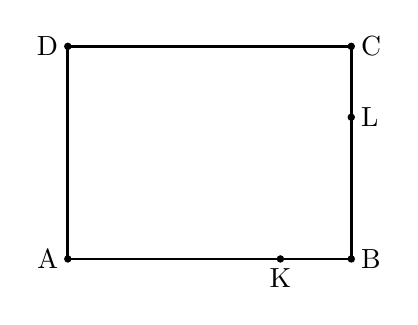
\begin{tikzpicture}[scale=0.9]
			\coordinate (A) at (0,0);
			\coordinate (B) at (4,0);
			\coordinate (C) at (4,3);
			\coordinate (D) at (0,3);
			\coordinate (K) at (3,0);
			\coordinate (L) at (4,2);
			\draw[line width=1pt] (A)--(B)--(C)--(D)--cycle;
			\fill (A) circle(1.5pt) node[left] {A};
			\fill (B) circle(1.5pt) node[right] {B};
			\fill (C) circle(1.5pt) node[right] {C};
			\fill (D) circle(1.5pt) node[left] {D};
			\fill (K) circle(1.5pt) node[below] {K};
			\fill (L) circle(1.5pt) node[right] {L};
		\end{tikzpicture}
	\end{center}

	\textbf{Affirmation :} le produit scalaire $\vectt{KD} \cdot \vectt{KL}$ est égal à $3$.
\end{enumerate}
